\section{Auswahl einer geeigneten Untermenge an Variablen}

\subsection{Vorgehen}
Um eine geeignete Untermenge an Variablen für die multivariate Analyse zu finden, haben wir die Relevanz der
Variablen, die je nach verwendetem Trainingsalgorithmus (Likelihood, Fisher, BDT, MLP) unterschiedlich ausfallen kann, evaluiert. Hierzu haben wir verschiedene Verfahren angewandt, die im Folgenden beschrieben werden.


Im Zuge der  Ausführung der Trainingsalgorithmen des vorgegebenen TMVA-Templates wird von diesem für jede Klassifizierungsmethode eine Rangliste bzgl. der Wichtigkeit der einzelnen Variablen erstellt. Um die Tauglichkeit dieser Rangliste zu überprüfen, betrachteten wir die Trainingsalgorithmen separat und trainierten den Likelihood-, Fisher-, sowie den BDT-Algorithmus jeweils insgesamt 30 mal, wobei entsprechend der vom TMVA-Template ausgegebenen Reihenfolge jeweils eine Variable entfernt wurde (beginnend mit der irrelevantesten).Bei jedem dieser insgesamt 90 Trainings wurde der ausgegebene AMS-Wert für das entsprechende Variablen-Subset protokolliert. Die Entwicklung der AMS-Werte mit abnehmender Variablenzahl sind in Abbildung \ref{fig:ams_over_parameter_count} gezeigt. Es ist deutlich zu erkennen, dass der Likelihood-Algorithmus einen ähnlichen Verlauf wie der Fisher-Algorithmus aufweist. Dies lässt sich dadurch erklären, dass es sich hierbei um ähnliche Algorithmen handelt. Eine sinnvolle Untermenge an Variablen liese sich demnach mithilfe des Maximums des AMS-Verlaufs bestimmen.

Da das Training des neuronalen Netzwerks mit Abstand die meiste Zeit benötigt, wurde hier ein anderes Verfahren angewandt: Es wurden 30 Trainingsläufe mit je einer entfernten Variablen durchgeführt und die Variablen entsprechend des jeweils erreichten AMS-Werts sortiert. Anschließend führten wir das zuvor beschriebene Verfahren gemäß dieses Rankings durch und erhielten den in Abbildung \ref{fig:ams_over_parameter_count} gezeigten Verlauf der AMS-Werte.


Dieses Verfahren stellte den Startpunkt für eine tiefergehende Analyse der Relevanz der einzelnen Variablen dar: Für jede Methode wurde das Training 30 mal mit jeweils einer aus dem Parameterset entfernten Variable durchgeführt, wobei die irrelevanteste Variable (höchster AMS-Wert) ermittelt wurde. Diese wurde aus dem Variablen-Set entfernt und das Training 29 mal durchgeführt, wobei jeweils eine der übrigen Variablen entfernt wurde. Je nach erzieltem AMS-Wert wurde das Parameter-Subset wiederum um den unwichtigsten Parameter reduziert usw. Da dieses Vorgehen aufgrund der langen Trainingszeit des neuronales Netzwerks hierfür nicht durchzuführen war, beschränkten wir uns hierbei auf die übrigen drei Verfahren. Insgesamt wurde zur Erstellung der entsprechenden Rankings das Training $3\cdot465=1395$ mal durchgeführt. Der Verlauf des AMS-Werts in Abhängigkeit der Anzahl verwendeter Parameter ist  Abbildung \ref{fig:ams_over_parameter_count} zu entnehmen. Da die AMS-Werte höher liegen als bei dem zuvor beschriebenen Verfahren, ist diese Rangliste als aussagekräftiger zu erachten.


\subsection{Auswertung}

Die Ergebnisse für den Verlauf der AMS-Werte bzgl. der verschiedenen Ranglisten sind in Abbildung \ref{fig:ams_over_parameter_count} gezeigt. Ein senkrechter Strich markiert jeweils das Maximum, anhand dessen die Auswahl des geeigneten Variablen-Subsets festgelegt wurde: Alle Variablen, die zu diesem Zeitpunkt noch Teil des Trainingsprozesses waren, sind Teil des für die weitere Auswertung der Daten gewählten Parameter-Sets. Welche Variablen dies für die jeweiligen Trainings-Algorithmen sind, ist Tabelle \ref{table:parameter_ranking} zu entnehmen. An oberster Stelle in der Tabelle stehen dabei die für die Analyse wichtigsten Parameter. Ein waagrechter Strich zeigt die Begrenzung des Variablen-Subsets an. 

Eine deutliche Verbesserung des AMS-Werts durch eine Verkleinerung der Variablenanzahl zeigt sich lediglich bei der Likelihood-Methode (siehe Abbildung \ref{fig:ams_over_parameter_count}). Da allerdings hiermit auch eine Reduzierung der Trainingszeit einhergeht, was vor allem beim neuronalen Netzwerk aufgrund seiner langen Algorithmenlaufzeit vorteilhaft ist.


%\usepackage{graphics} is needed for \includegraphics
\begin{figure}[htp]
\begin{center}
  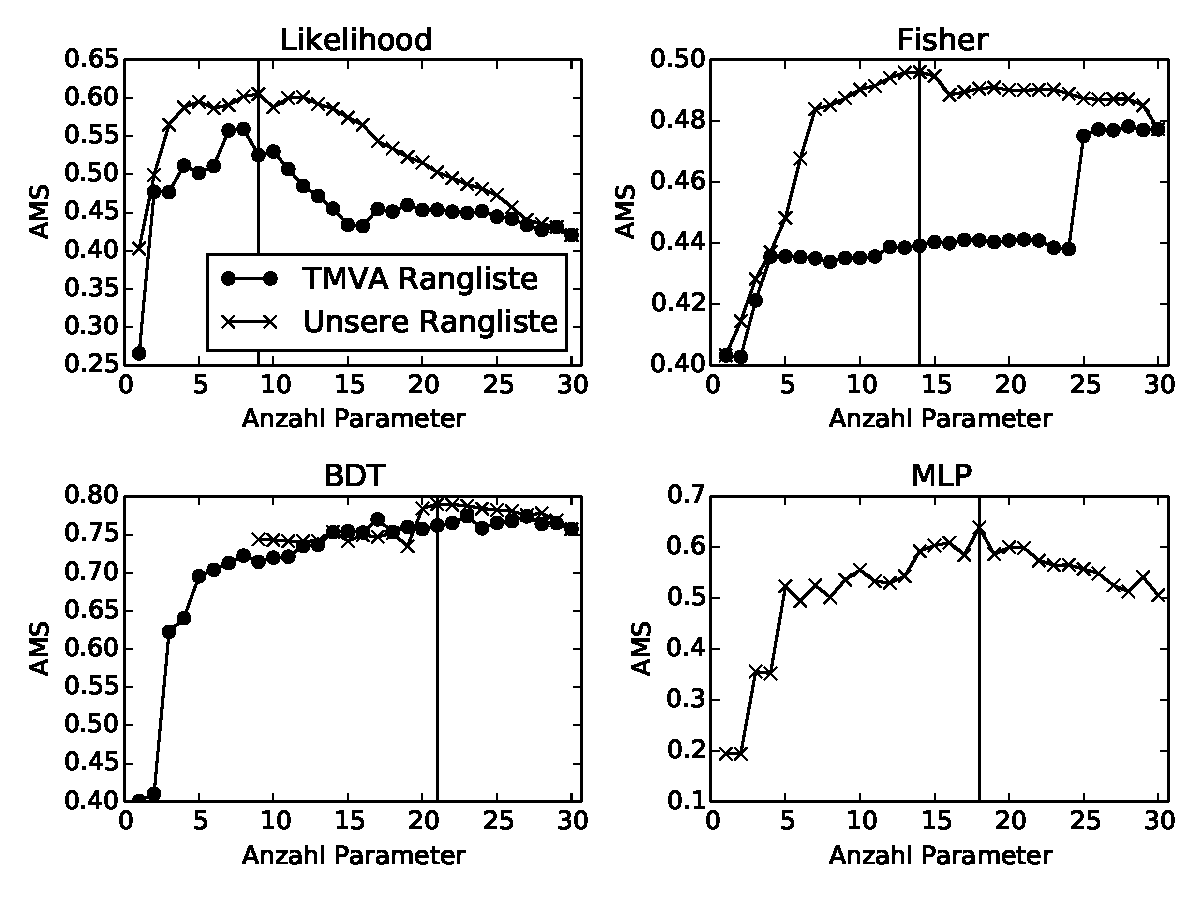
\includegraphics[width=\linewidth]{sections/subset_of_parameters/parameter_count_ranking_by_method.pdf}
  \caption[AMS über der Anzahl der Parameter]{AMS über der Anzahl der Variablen.}
  \label{fig:ams_over_parameter_count}
\end{center}
\end{figure}

\begin{table}
\caption{Rangliste der Variablen bzgl. ihrer Relevanz für die Analyse. Die Wichtigkeit der Parameter nimmt von oben nach unten ab. Für jede Methode ist durch einen waagrechten Strich die durch das Maximum des AMS-Verlaufs gegebene Abgrenzung einer geeigneten Auswahl an Variablen gekennzeichnet. Bei der BDT-Methode wurde unter den besten acht Parametern kein Ranking vorgenommen.}
\small
\hspace{-1cm}
\begin{tabular}{c|c|c|c}
Likelihood & Fisher & BDT & MLP \\
\hline
d\_mass\_transverse\_met\_lep & d\_mass\_transverse\_met\_lep & - & p\_jet\_num
\\
d\_mass\_vis & d\_pt\_ratio\_lep\_tau & - & d\_deltaeta\_jet\_jet \\ 
p\_tau\_pt & p\_lep\_pt & - & d\_mass\_MMC \\ 
d\_deltar\_tau\_lep & d\_mass\_vis & - & p\_jet\_leading\_pt \\ 
d\_pt\_ratio\_lep\_tau & d\_deltar\_tau\_lep & - & d\_mass\_transverse\_met\_l \\ 
p\_met & d\_pt\_h & - & p\_jet\_leading\_eta \\ 
p\_lep\_pt & p\_tau\_pt & - & d\_mass\_jet\_jet \\ 
p\_lep\_eta & d\_mass\_jet\_jet & - & p\_jet\_leading\_phi \\ 
d\_mass\_MMC & p\_met & d\_mass\_MMC & d\_pt\_h \\ 
----- & & & \\ 
p\_jet\_leading\_phi & d\_prodeta\_jet\_jet & d\_lep\_eta\_centrality & d\_mass\_vis \\ 
d\_met\_phi\_centrality & p\_jet\_subleading\_pt & p\_jet\_subleading\_phi & p\_jet\_subleading\_phi \\ 
p\_tau\_phi & p\_lep\_phi & p\_tau\_pt & d\_prodeta\_jet\_jet \\ 
p\_met\_phi & d\_mass\_MMC & d\_mass\_vis & p\_jet\_subleading\_pt \\ 
p\_tau\_eta & d\_deltaeta\_jet\_jet & p\_tau\_phi & p\_tau\_pt \\ 
 & ----- & & \\ 
p\_jet\_subleading\_pt & d\_lep\_eta\_centrality & p\_met\_sumet & p\_met\_phi \\ 
d\_pt\_tot & p\_jet\_leading\_phi & p\_lep\_pt & p\_jet\_all\_pt \\ 
p\_jet\_subleading\_eta & p\_jet\_leading\_eta & p\_lep\_phi & p\_met\_sumet \\ 
d\_prodeta\_jet\_jet & d\_sum\_pt & p\_jet\_subleading\_pt & p\_tau\_eta \\ 
 & & & ----- \\ 
p\_jet\_subleading\_phi & p\_jet\_subleading\_eta & p\_jet\_subleading\_eta & p\_met \\ 
p\_met\_sumet & p\_tau\_phi & d\_pt\_tot & d\_met\_phi\_centrality \\ 
d\_deltaeta\_jet\_jet & p\_met\_phi & p\_jet\_subleading\_eta & d\_pt\_ratio\_lep\_tau \\ 
 & & ----- & \\ 
d\_mass\_jet\_jet & p\_jet\_leading\_pt & p\_jet\_subleading\_phi & p\_tau\_phi \\ 
d\_lep\_eta\_centrality & p\_tau\_eta & p\_jet\_subleading\_pt & p\_jet\_subleading\_eta \\ 
p\_lep\_phi & p\_met\_sumet & d\_pt\_h & p\_lep\_phi \\ 
p\_jet\_num & p\_jet\_num & p\_met & d\_pt\_tot \\ 
d\_pt\_h & d\_pt\_tot & d\_prodeta\_jet\_jet & p\_lep\_eta \\ 
d\_sum\_pt & p\_lep\_eta & p\_lep\_pt & d\_sum\_pt \\ 
p\_jet\_leading\_pt & p\_jet\_subleading\_phi & d\_pt\_tot & d\_lep\_eta\_centrality \\ 
p\_jet\_all\_pt & p\_jet\_all\_pt & p\_met\_phi & p\_lep\_pt \\ 
p\_jet\_leading\_eta & d\_met\_phi\_centrality & p\_lep\_phi & d\_deltar\_tau\_lep

\end{tabular}
\label{table:parameter_ranking}
\end{table}